\documentclass[10pt,aspectratio=43]{beamer}

\usepackage{graphicx}
\usepackage{tikz}
\usepackage{xcolor}
\usepackage{caption}
\usepackage{subcaption}
\usepackage{bm}
\usetikzlibrary{calc} 
\usepackage{hyperref}
\hypersetup{
    colorlinks=true,
    linkcolor=blue,
    urlcolor=red
}
\usepackage{fontawesome5}
\usepackage{ulem}
\usepackage[dvipsnames]{xcolor}

\usetheme{MyStyle}   % loads beamerthemeMyStyle.sty
\setlength{\columnsep}{0pt}


%%%%%%%%%%%%%%%%%%%%%%%%%%%%%%%%%%%%%%%%%%
%%%%%%%%%%%%%%%%%%%%%%%%%%%%%%%%%%%%%%%%%%
%%%%%%%%%%%%%%%%%%%%%%%%%%%%%%%%%%%%%%%%%%

\title{Time reconstruction of saturated signals}
\newcommand{\eventname}{CALCOM meeting}
\author{Felix Touchte Codjo}
\institute{IJCLab}
\date{\today}


\begin{document}

\begin{frame}[plain] % remove header, footer, barre de navigation
\titlepage
\end{frame}

%\begin{frame}{Outline}
%\tableofcontents
%\end{frame}

%\section{Intro}
\section{Updates}



\begin{frame}{Current situation}
    \begin{itemize}
        \item The time of arrival is extracted at half the amplitude
        \item For saturated signals, this creates a bias
            \begin{itemize}
                \item The reconstructed time is under-estimated
                \item This will impact track reconstruction of $\alpha$ particles
                \item Some hits may not even pass selection cuts and tracks can be lost
            \end{itemize}
        \item This study aims to reconstruct a corrected time
            \begin{itemize}
                \item The first step is to reconstruct the ADC of the saturated signals
            \end{itemize}
    \end{itemize}

    \centering
    \vspace{0.2cm}

    \begin{figure}
        \includegraphics[width=0.55\linewidth]{figures/build/isssue-time-of-saturated-signals.pdf}
    \end{figure}

\end{frame}




\begin{frame}{Finding the good method}
    \begin{itemize}
        \item We look at two options 
            \begin{itemize}
                \item Time over threshold (ToT) or maximum of the leading edge slope
                \item We compare the two methods using non-saturated signals
                \item We look at how correlated the variables are to the ADC
            \end{itemize}
        \item The ToT as a function of the ADC is not linear
            \begin{itemize}
                \item This might be an issue as we need to extrapolate to much larger values
            \end{itemize}
        % \textit{\textbf{(ii)}} it is more precise than the slope at low ADC, \textit{\textbf{(iii)}} but the resolution increases with the ADC while it is almost constant in the slope method
    \end{itemize}

    \centering
    \vspace{0.2cm}

    {   \setlength{\tabcolsep}{2pt}
        \begin{tabular}{cc}
            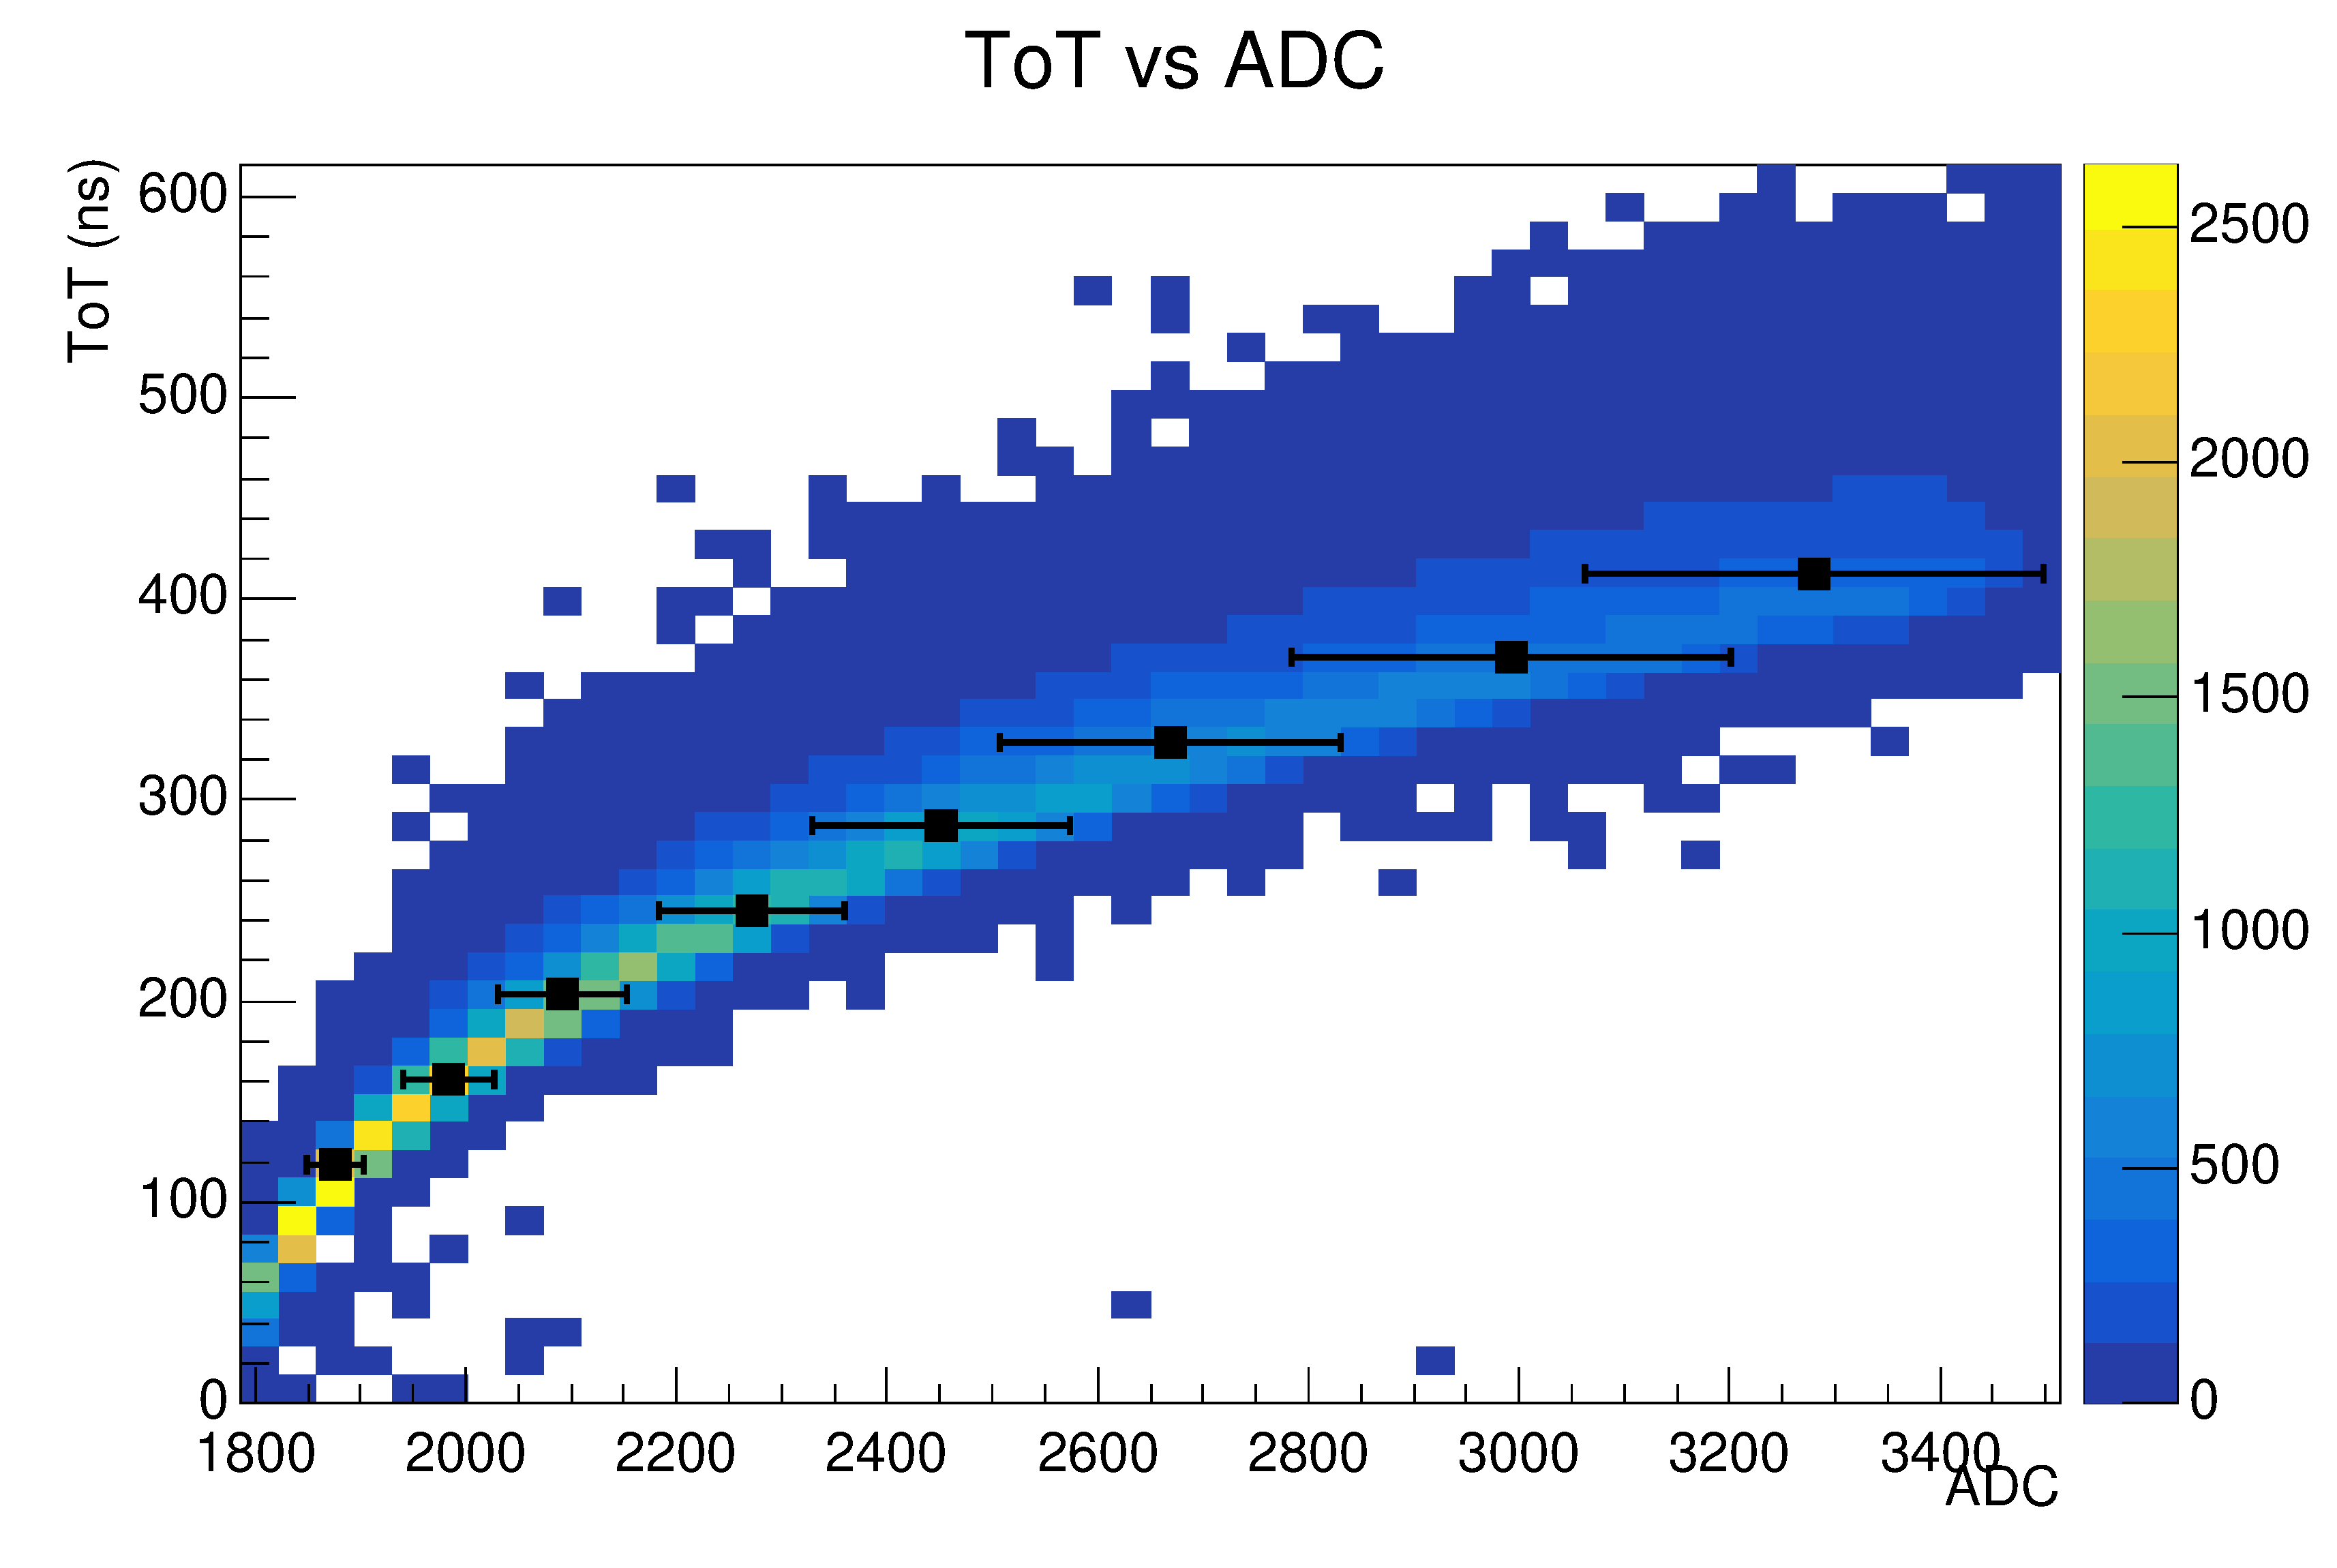
\includegraphics[width=0.48\linewidth]{figures/validation-tot-vs-adc.pdf} &
            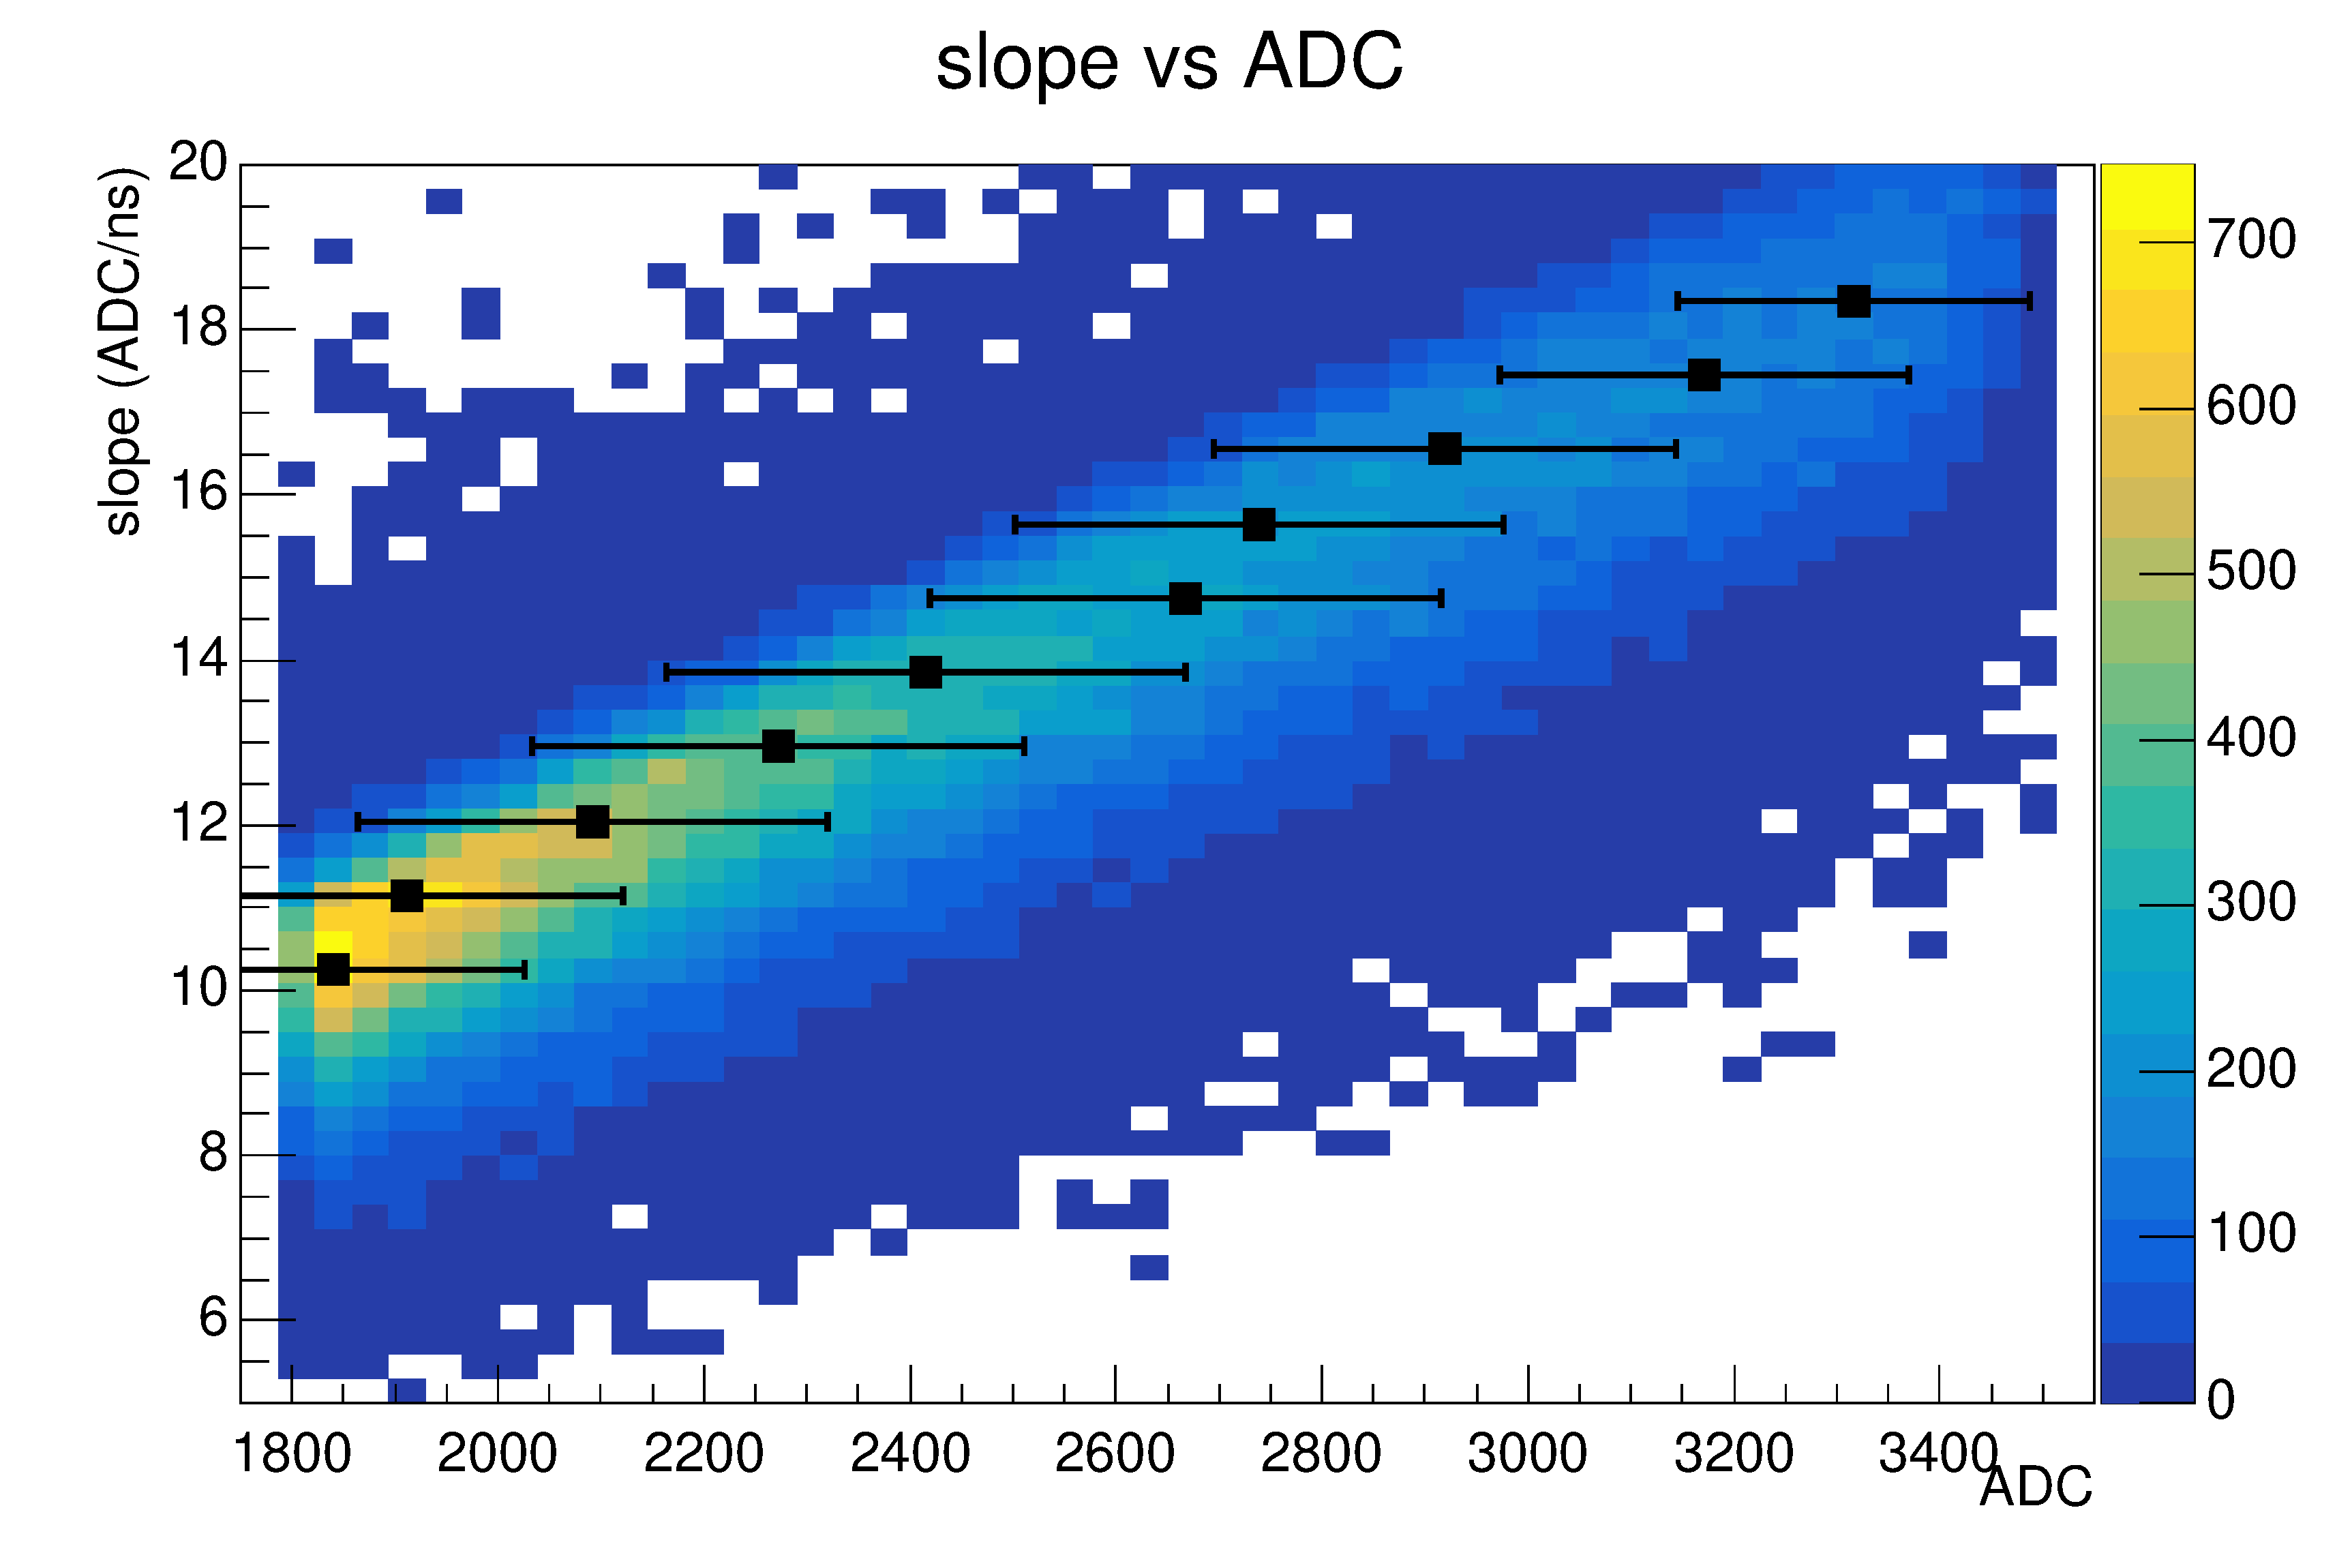
\includegraphics[width=0.48\linewidth]{figures/validation-slope-vs-adc.pdf} \\
        \end{tabular}
    }
\end{frame}

\begin{frame}{Comparison of the resolutions}

    \begin{itemize}
        \item We plot the error obtained in the previous slide
            \begin{itemize}
                \item The slope method has a constant error
                \item The ToT has a growing error
            \end{itemize}
        \item We choose to use the maximum slope method
            \begin{itemize}
                \item Its linear behavior will be much easier to extrapolate
                \item At larger ADC, the precision will likely be better
                \item Large signals are often missing their trailing edge
            \end{itemize}
    \end{itemize}

    \centering
    \vspace{0.2cm}

    \begin{figure}
        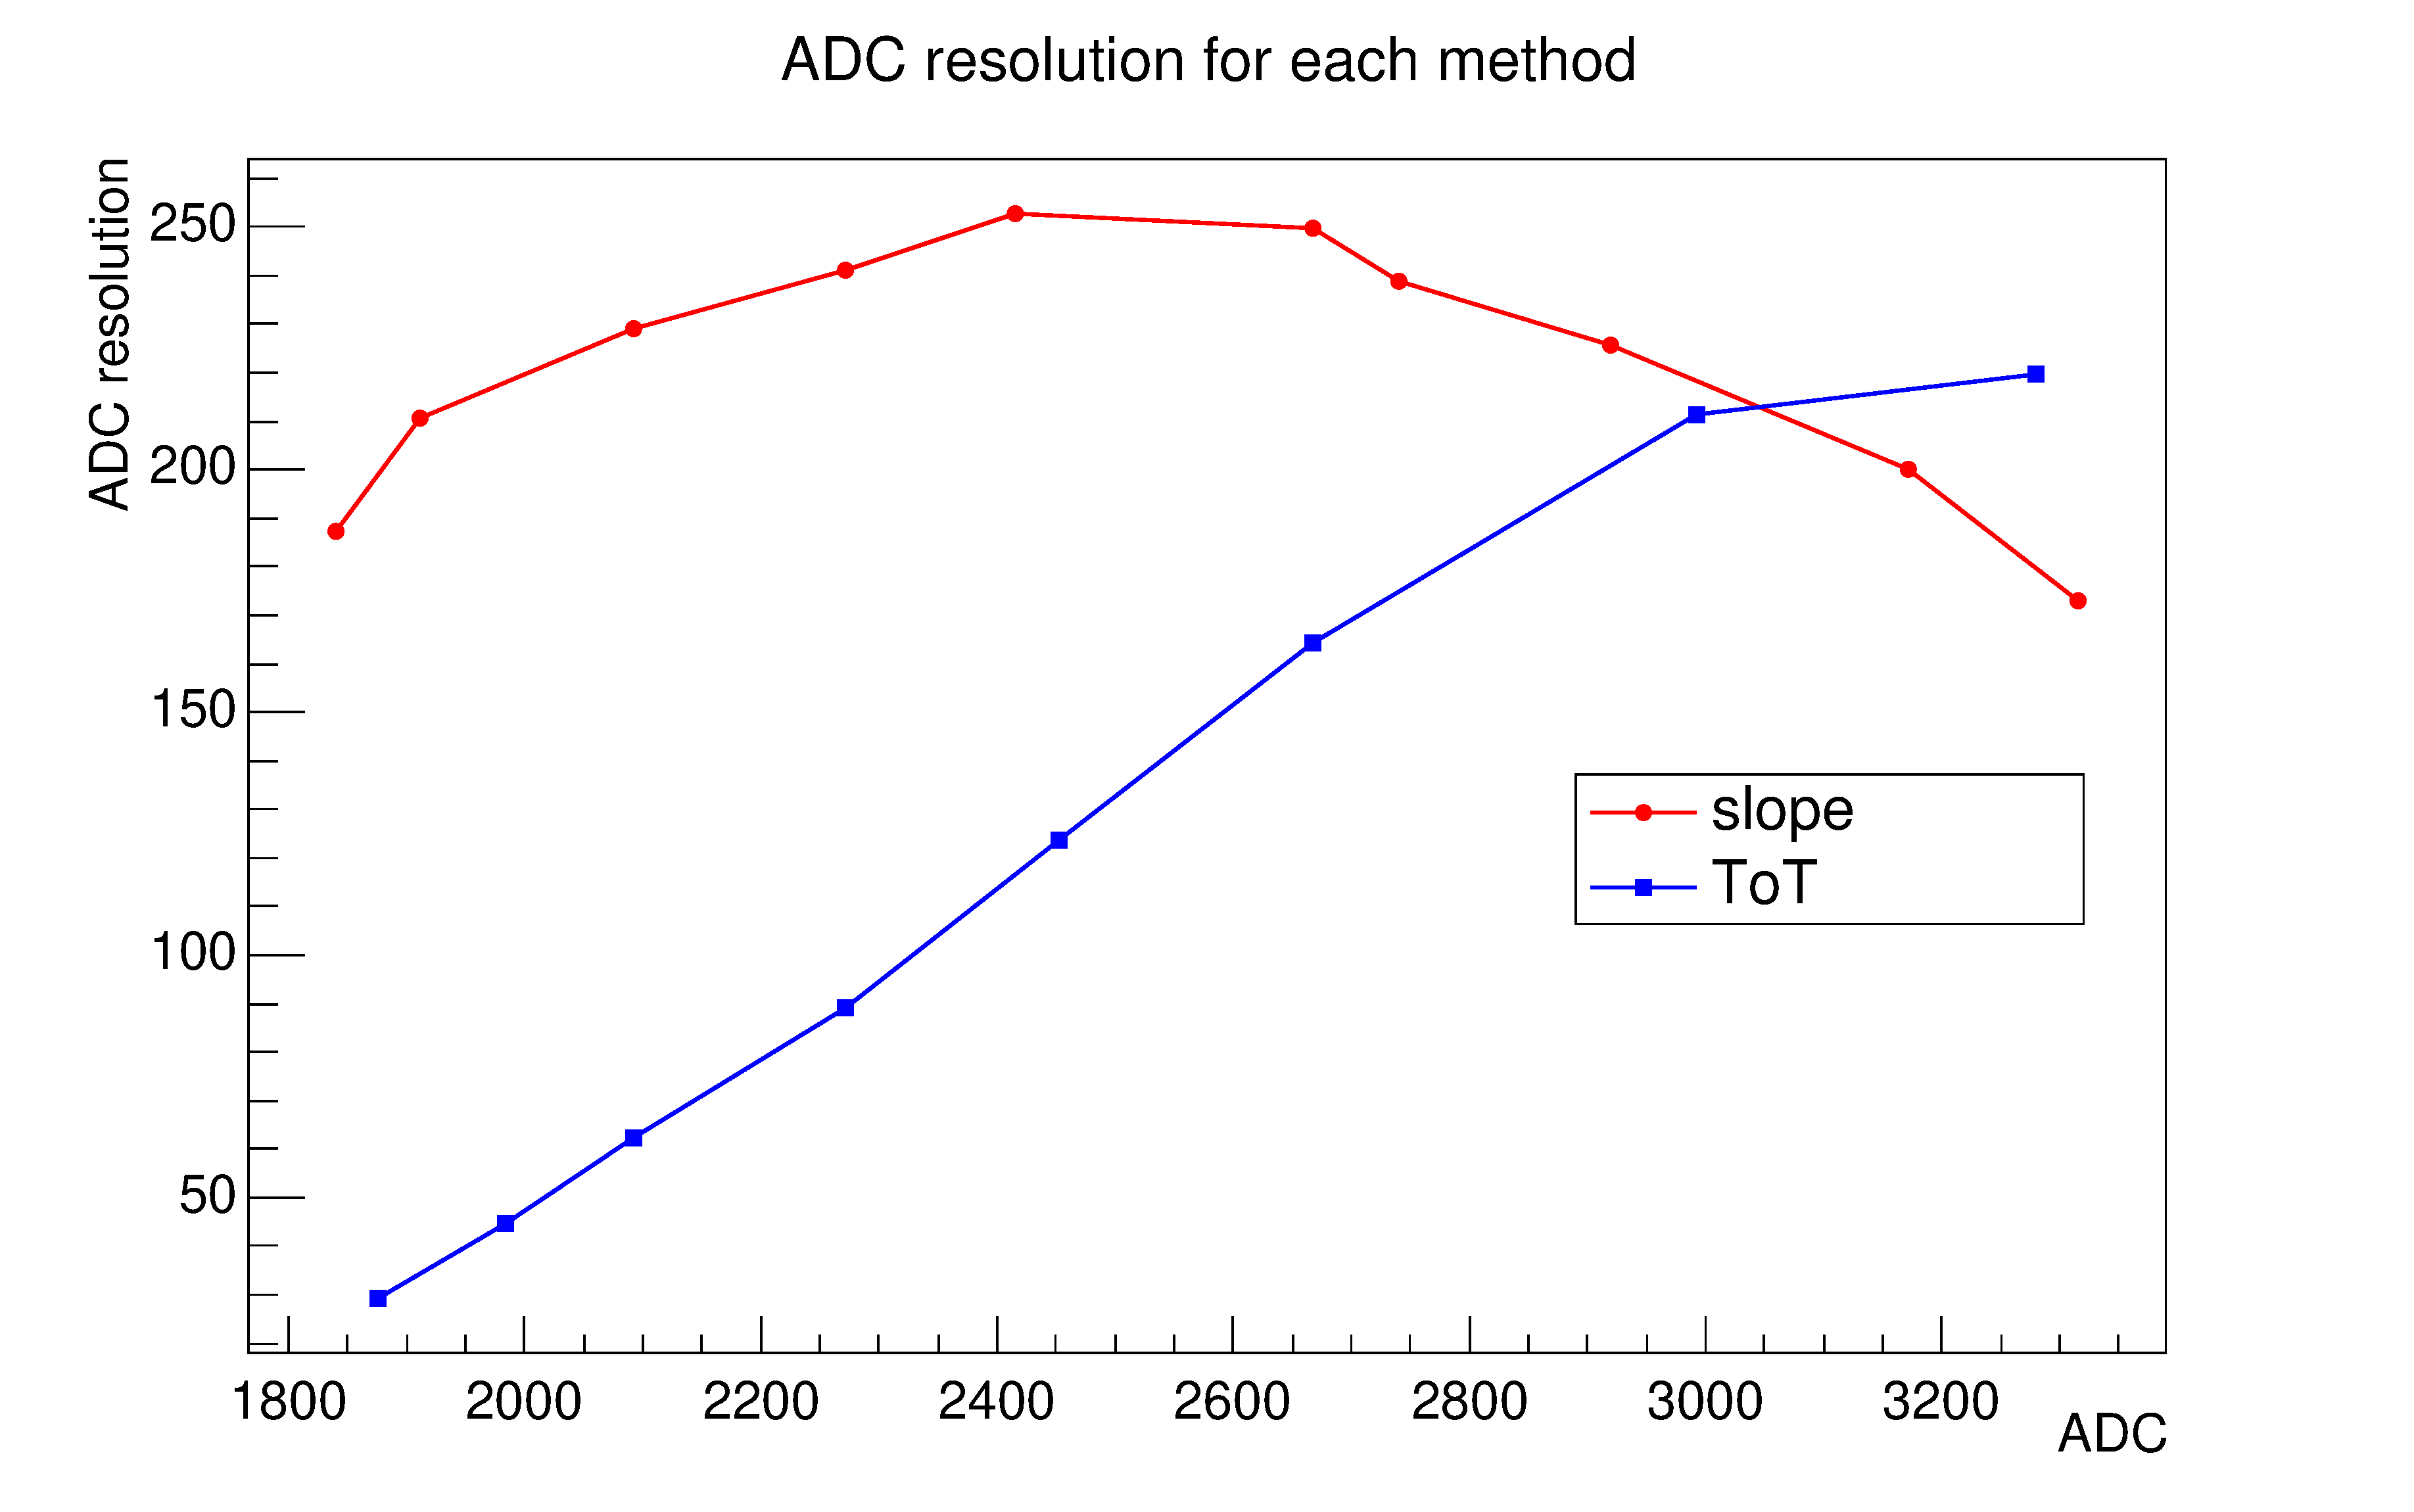
\includegraphics[width=0.65\linewidth]{figures/validation-adc-resolution-vs-method.pdf}
    \end{figure}
    
\end{frame}

\begin{frame}{Reconstructing the ADC}
    \begin{itemize}
        \item The maximum of the slope of the signal is linearly correlated to the amplitude of the signal
            \begin{itemize}
                \item Saturated hits seem to follow the trend
            \end{itemize}
        \item We can use the slope to estimate the amplitude of the signal
            \begin{itemize}
                \item We extract the ADC as a function of the slope from non-saturated signals and apply it to the saturated ones
            \end{itemize}
    \end{itemize}

    \centering
    \vspace{0.2cm}

    \begin{tabular}{cc}
        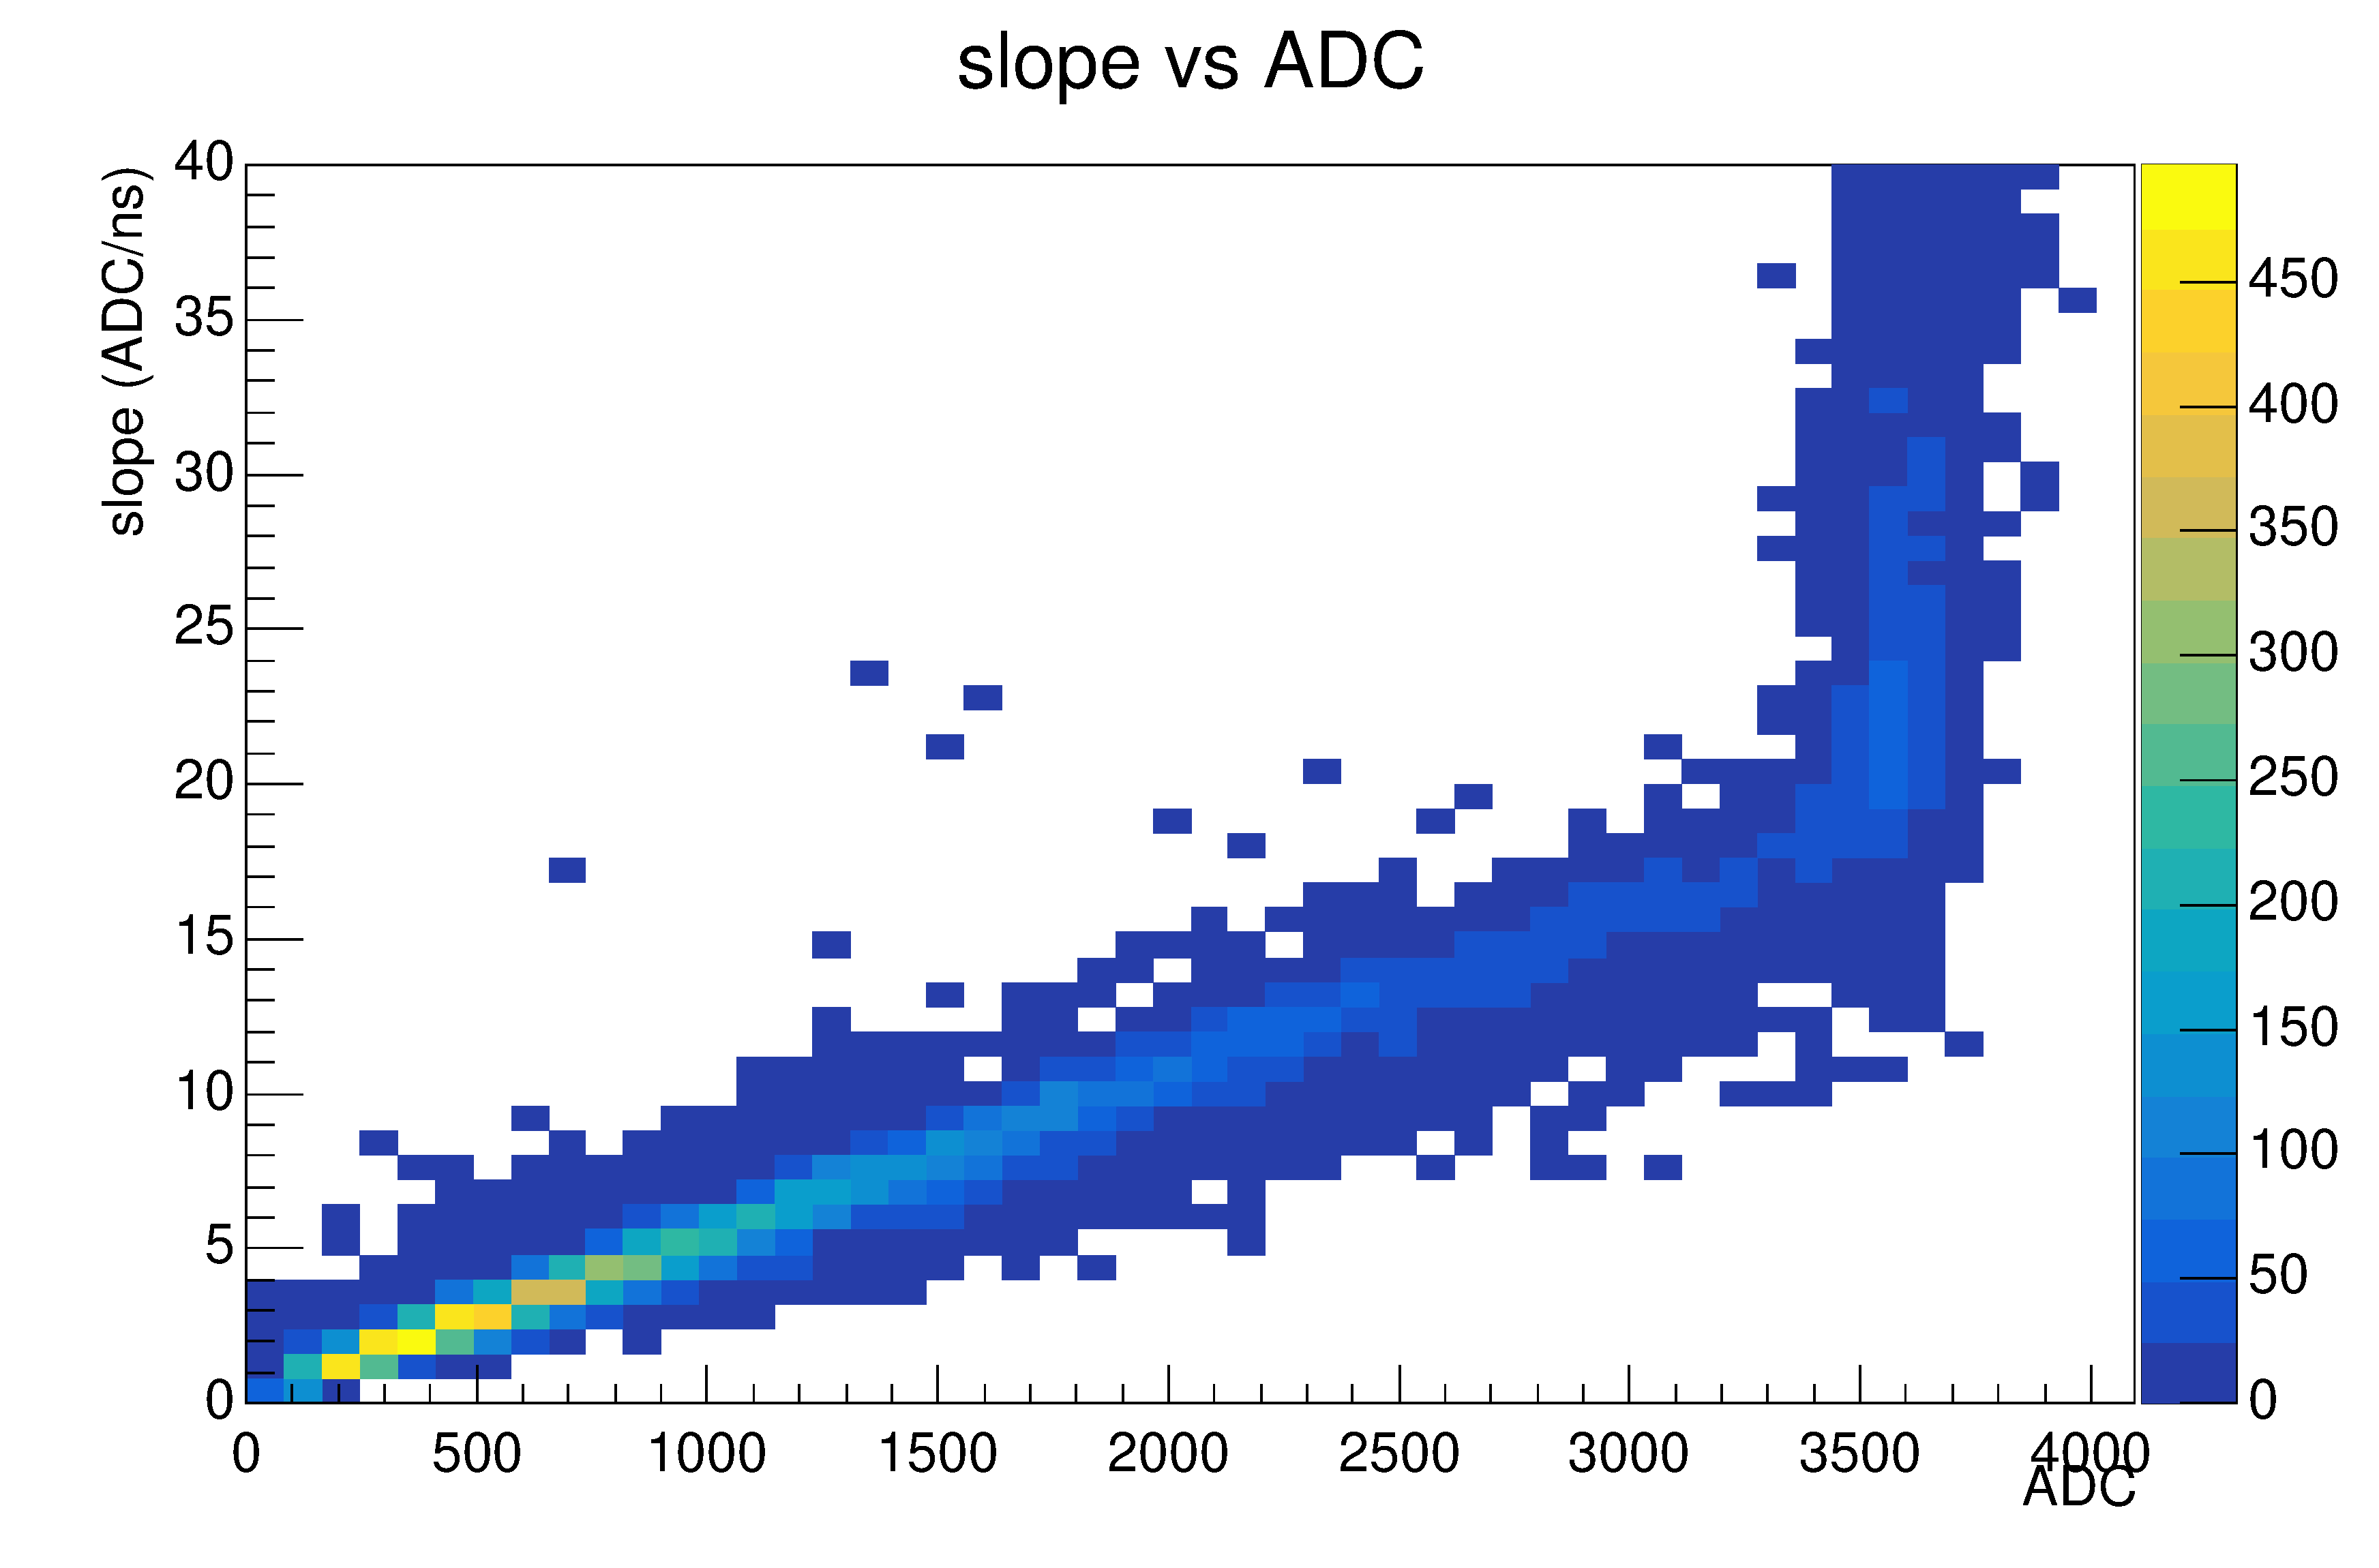
\includegraphics[width=0.48\linewidth]{figures/slope-versus-adc-all-signals.pdf} &
        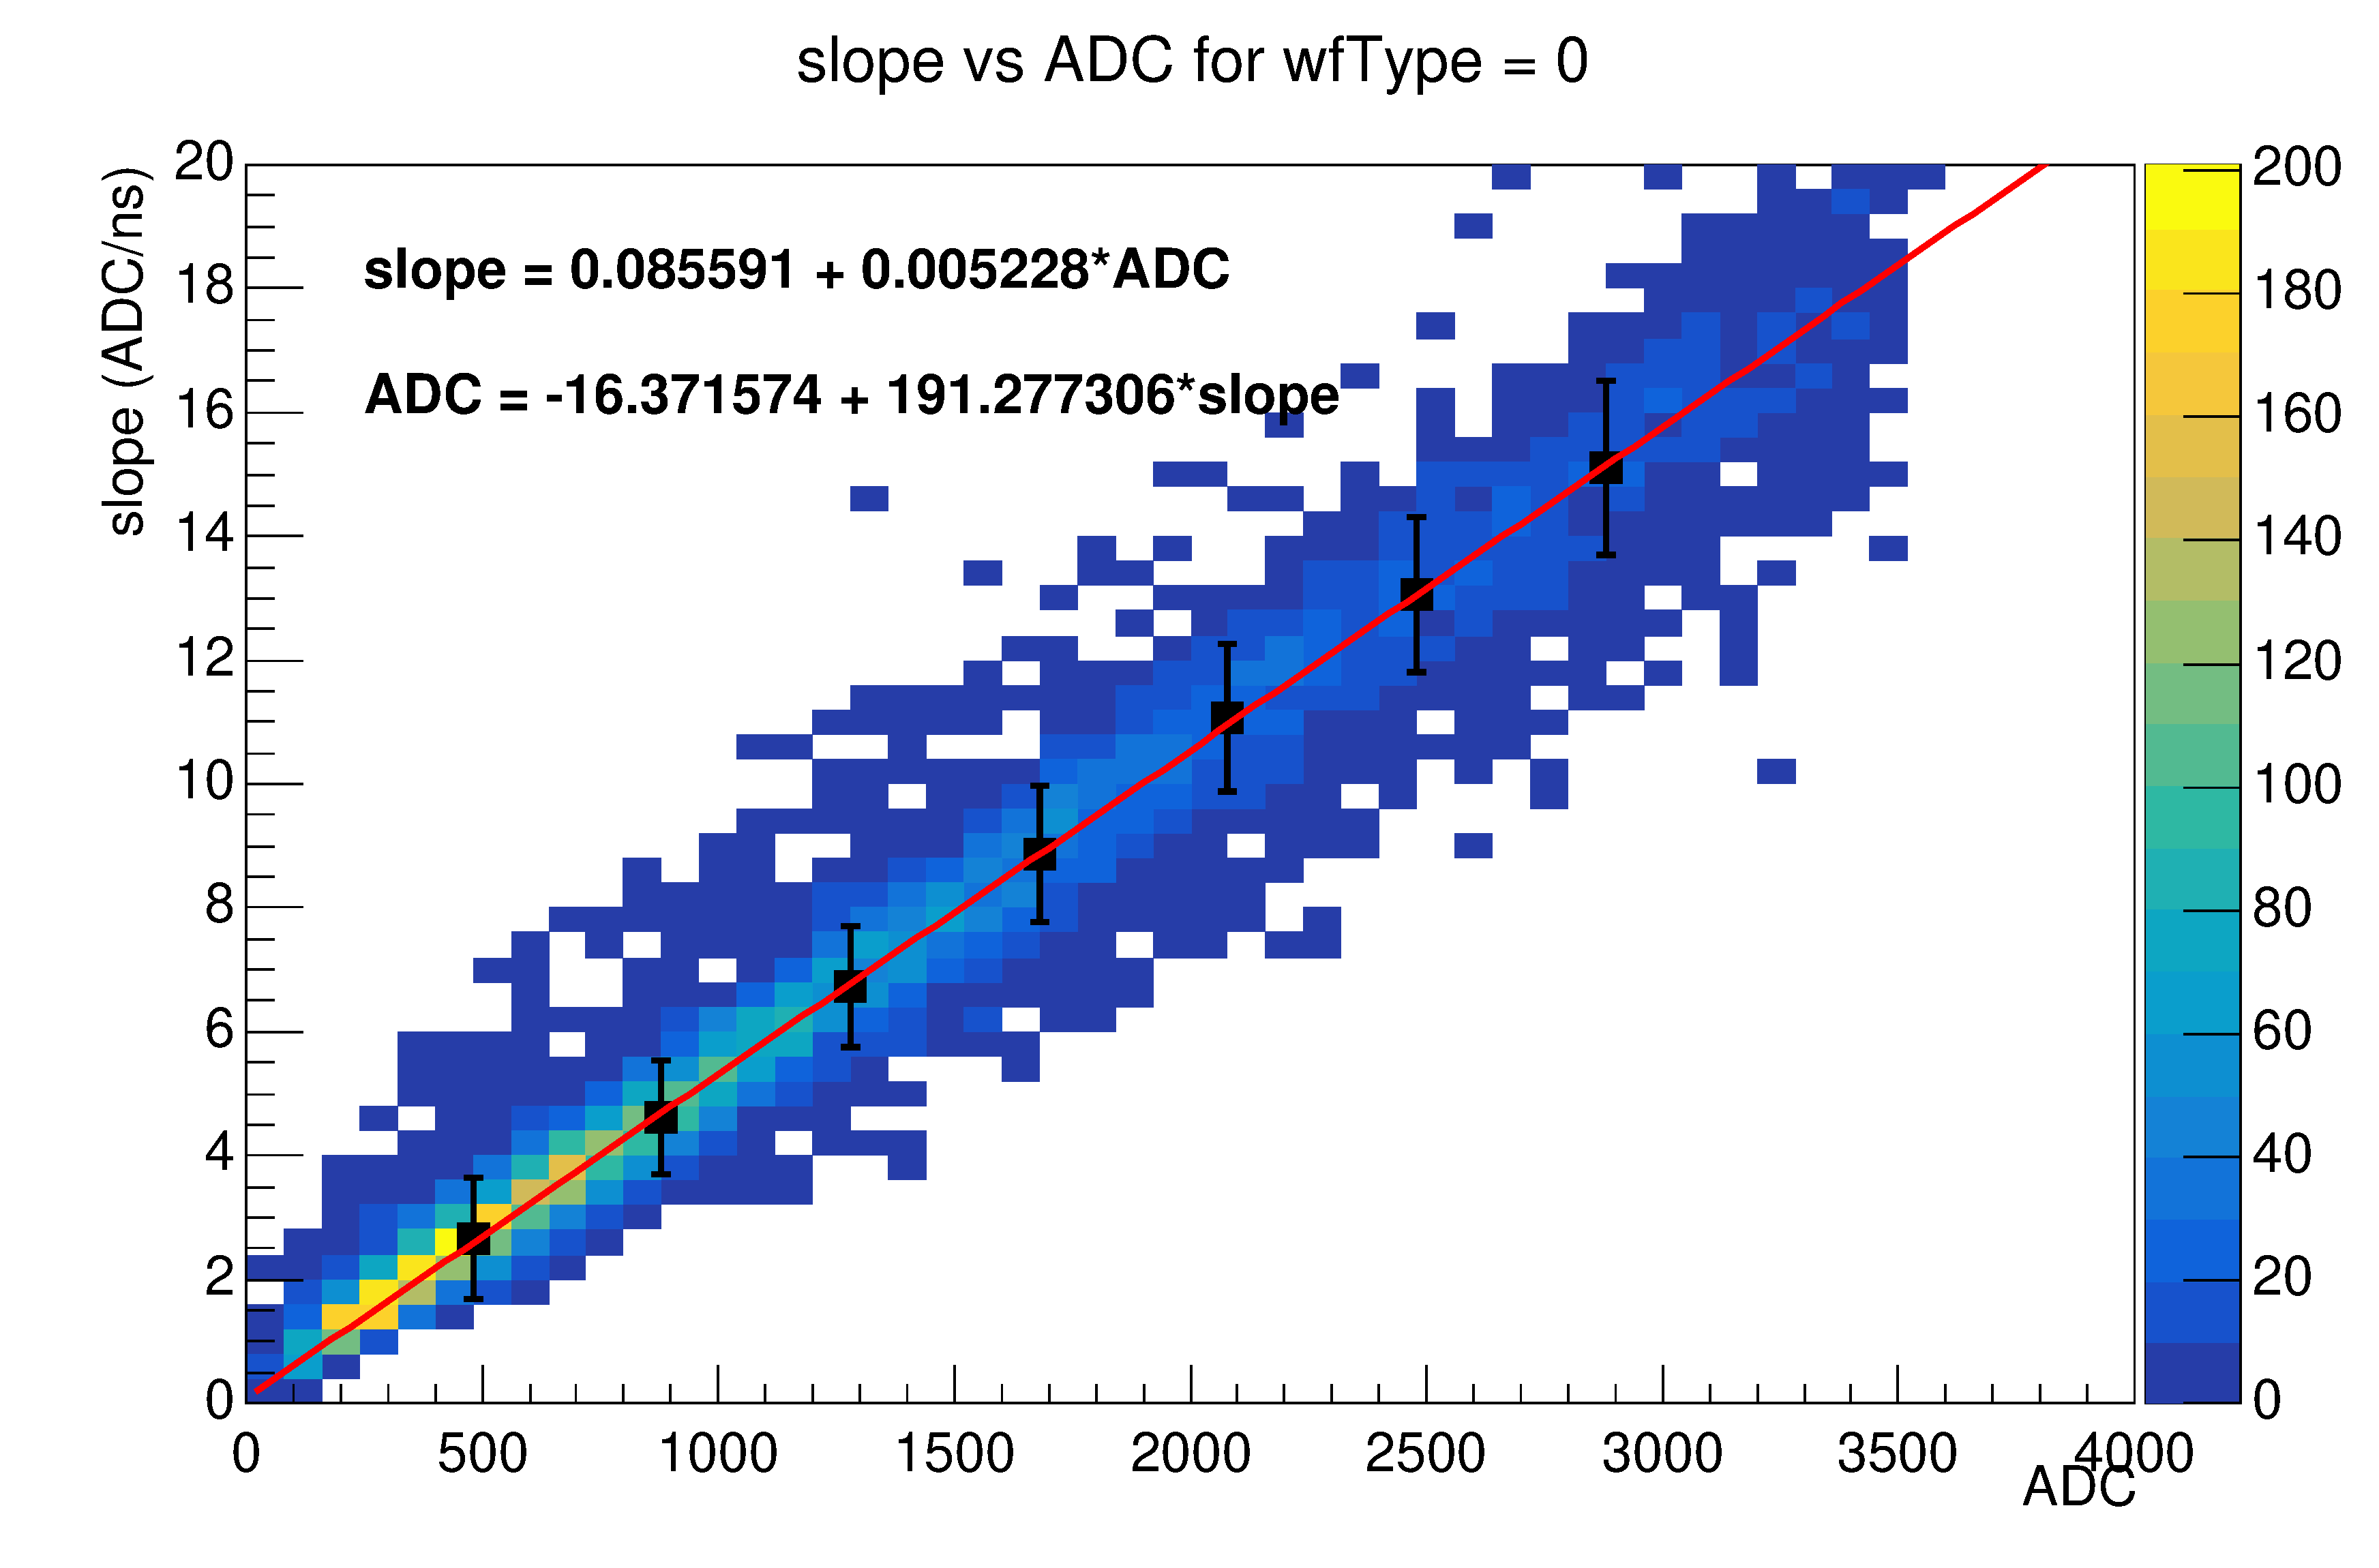
\includegraphics[width=0.48\linewidth]{figures/slope-versus-adc-wfType0.pdf} 
    \end{tabular}
    
\end{frame}

\begin{frame}{Time reconstruction}
    \begin{itemize}
        \item With the corrected amplitude, we can recompute the time
            \begin{itemize}
                \item We use the time at half the corrected ADC
                \item However, sometimes even half ADC is above the saturation threshold
                \item In this case, we extrapolate the signal based on the maximum slope to determine the time at half ADC
                % \item The error of the estimation is well known and is propagated to the reconstructed time 
                % \item The big slope of saturated signals make the error on the time very minimal
                % \item The error on the time can be propagated to the DOCA and provided to the Kalman Filter
            \end{itemize}
        %\item 
    \end{itemize}

    \centering
    \vspace{0.2cm}

    % \begin{figure}
    %     \includegraphics[width=0.55\linewidth]{figures/build/isssue-time-of-saturated-signals_decoding.pdf}
    % \end{figure}

    {   \setlength{\tabcolsep}{2pt}
        \renewcommand{\arraystretch}{0.5}
        \begin{tabular}{cc}
            \includegraphics[width=0.48\linewidth]{figures/build/isssue-time-of-saturated-signals_decoding.pdf} &
            \includegraphics[width=0.48\linewidth]{figures/build/isssue-time-of-saturated-signals_decoding_case2.pdf} \\
            \footnotesize 1/2 ADC below saturation & \footnotesize 1/2 ADC above saturation \\
            \footnotesize (direct interpolation) & \footnotesize (use the slope to extrapolate)
        \end{tabular}
    }
\end{frame}

\begin{frame}{Results - Effect of the correction}
    \begin{itemize}
        \item Before correction
            \begin{itemize}
                \item We had an accumulation of hits around 3600 ADC
                \item Saturated hits had abnormal tail in the low time direction
            \end{itemize}
        \item After correction
            \begin{itemize}
                \item We reconstruct ADCs above saturation 
                \item There are no more hit accumulation at low time and large amplitude
                \item We move from 2244 reconstructed tracks to 2436
                    \begin{itemize}
                        \item[$\rightarrow$] Using 10 files of run 21476, on 4He at 10.6 GeV
                        \item[$\rightarrow$] Most of the gained tracks have very high energy deposit
                    \end{itemize}
                
            \end{itemize}
        %\item Quantitatively, we move from 2244 reconstructed tracks to 2436 over 239852 selected trigger events in run 21476, so a gain of 8.55\%
    \end{itemize}

    \centering
    \vspace{0.2cm}

    {   \setlength{\tabcolsep}{2pt}
        \renewcommand{\arraystretch}{0.5}
        \begin{tabular}{cc}
            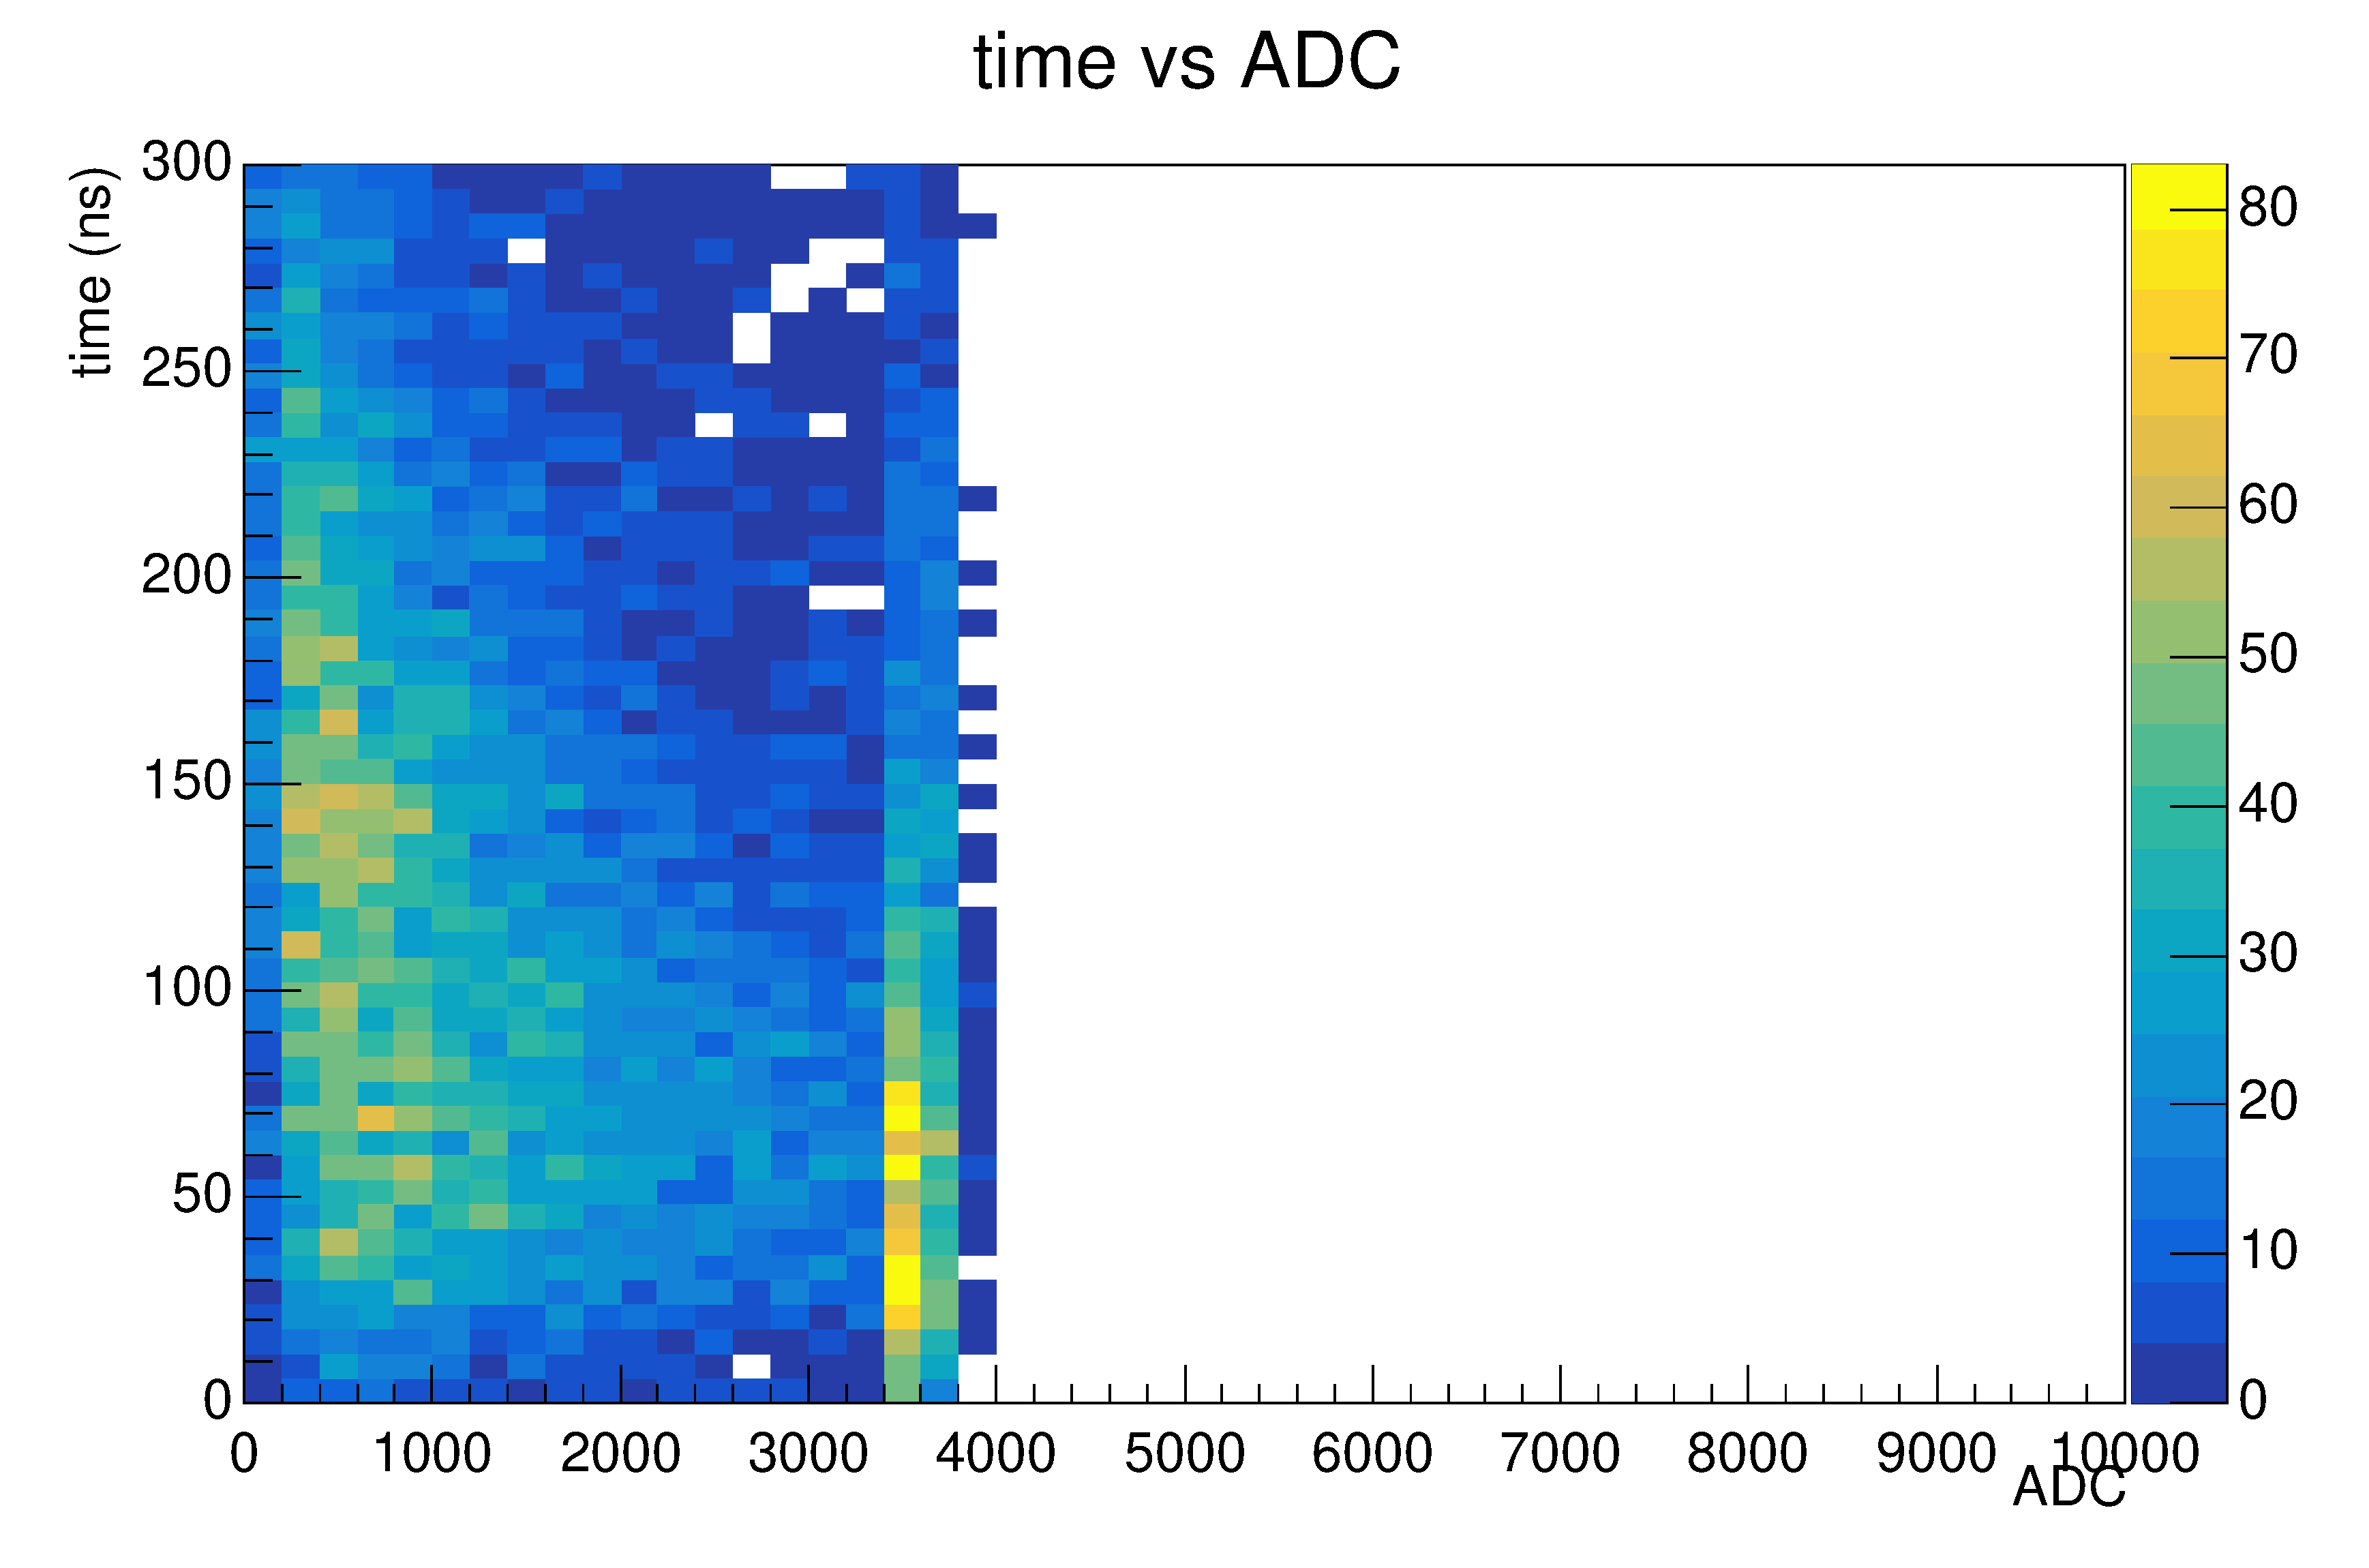
\includegraphics[width=0.48\linewidth]{figures/time-vs-adc-before-adc-correction.pdf} &
            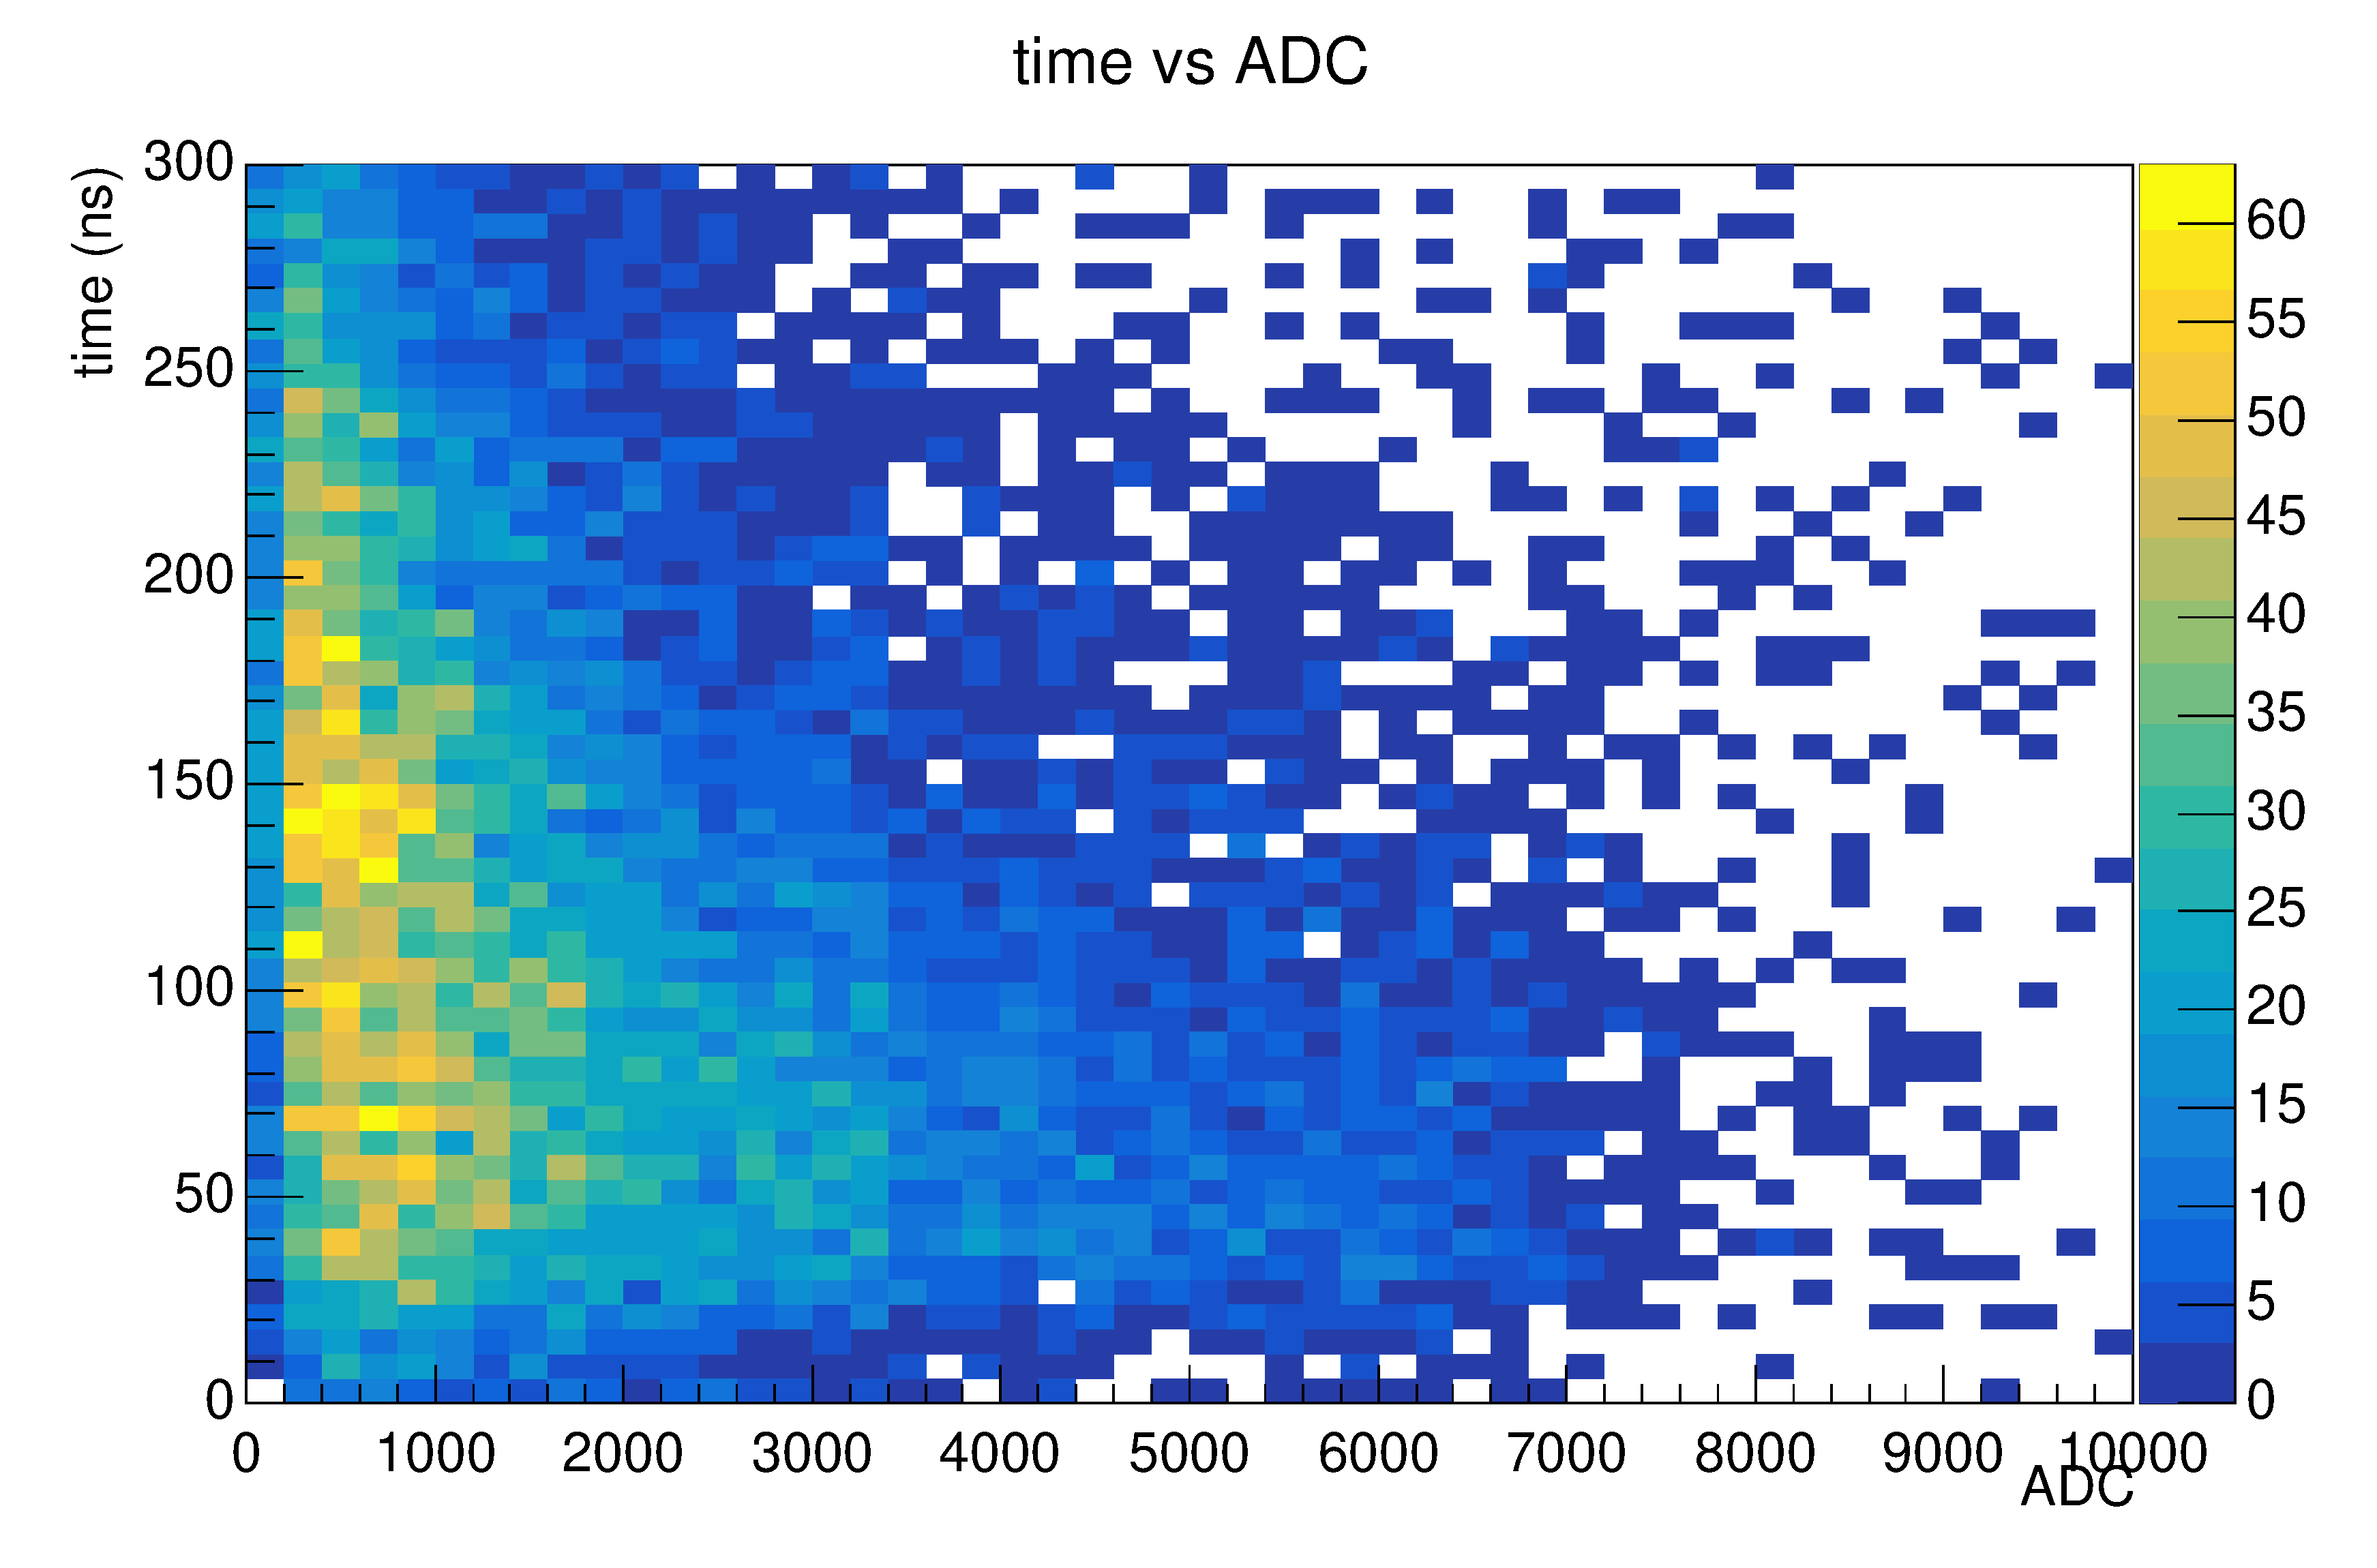
\includegraphics[width=0.48\linewidth]{figures/time-vs-adc-after-adc-correction.pdf} \\
            before & after \\
        \end{tabular}
    }

\end{frame}














\end{document}


